\documentclass[UTF8,a4paper,12pt]{ctexrep}

\usepackage{geometry}
\usepackage{booktabs}
\usepackage{tabularx}
\usepackage{longtable}
\usepackage{array}
\usepackage{enumitem}
\usepackage{hyperref}
\usepackage{xcolor}
\usepackage{listings}
\usepackage{amsmath}
\usepackage{tikz}
\usepackage{graphicx}
\usepackage{float}

\geometry{left=2.6cm,right=2.6cm,top=2.6cm,bottom=2.6cm}
\hypersetup{
  colorlinks=true,
  linkcolor=blue!50!black,
  urlcolor=blue!50!black,
  citecolor=blue!50!black
}

\setlist[itemize]{nosep,leftmargin=2em}
\setlist[enumerate]{nosep,leftmargin=2em}
\renewcommand{\arraystretch}{1.2}

\lstdefinestyle{codestyle}{
  basicstyle=\ttfamily\small,
  breaklines=true,
  frame=single,
  columns=fullflexible,
  keepspaces=true,
  keywordstyle=\color{blue!70!black},
  commentstyle=\color{green!40!black},
  stringstyle=\color{red!60!black}
}
\lstset{style=codestyle}

\title{\textbf{CourseCPU：RV32I 四级流水线处理器系统}\\
\large 设计、验证与 FPGA 实现报告}
\author{NullStarfish}
\date{\today}

\begin{document}

\maketitle
\tableofcontents

\chapter{CPU Overview}

CourseCPU 是一个完整的 RV32I 单发射、顺序执行、四级流水线 CPU 系统。它不是一个只服务于少量 directed test 的课堂 demo，而是一个能够运行真实 RISC-V ELF 程序、接入工业化仿真验证闭环、并可综合到 FPGA 的处理器原型。

CourseCPU 实现了 RV32I 整数指令级功能，并通过完整指令集回归测试、Verilator 周期级仿真以及基于 NEMU reference model 的 Differential Testing 进行验证。仿真框架支持由真实 RISC-V GCC 工具链编译得到的 ELF 程序，能够运行 \texttt{add-longlong}、\texttt{bubble-sort}、\texttt{quick-sort}、\texttt{recursion}、\texttt{select-sort} 等真实 C benchmark。项目同时提供基于 \texttt{abstract-machine} 的 C source SDK、ELF loader、交互式 SDB 调试器、commit trace、性能统计、flush 统计和调试基础设施。

\section{关键 PPA 与性能摘要}

\begin{table}[H]
  \centering
  \caption{CourseCPU 最终版本 PPA 与性能摘要}
  \begin{tabularx}{\textwidth}{lX}
    \toprule
    指标 & 结果 \\
    \midrule
    ISA / 微架构 & RV32I，单发射，顺序执行，四级流水线 \\
    Benchmark 加权 IPC & 0.799939（5 个真实 C benchmark，总 18305 条提交指令） \\
    Benchmark 平均 IPC & 0.829350（5 个 benchmark 算术平均） \\
    加权 Flush Probability & 8.3092\%（总 flush 1521 次） \\
    Timing / Fmax 估算 & 100 MHz 约束下 WNS = 1.255 ns，TNS = 0；按 $1000/(10-1.255)$ 估算 Fmax 约 114.35 MHz \\
    Utilization & 1796 LUT（22.45\%），1521 FF（9.51\%），0 BRAM，0 DSP \\
    Power & Total On-Chip Power = 0.113 W，其中 Dynamic = 0.054 W，Static = 0.059 W \\
    验证 & Verilator + Abstract-Machine + ELF loader + NEMU difftest + RTL readmemh testbench \\
    \bottomrule
  \end{tabularx}
\end{table}

在微架构上，CourseCPU 采用四级流水线组织，包括 IF、ID、EX、MEM/WB 四个阶段。处理器包含 Fetch 级 GShare Branch Predictor、数据相关 forwarding 网络、load-use hazard 处理、控制冒险 flush 机制、byte-addressed 数据存储器接口，以及面向仿真和 FPGA 综合的可配置裁剪机制。对于 Course 配置，CPU 裁剪了课程环境不需要的 CSR/SYS 路径，同时保留适合仿真退出与测试框架集成的 \texttt{sim ebreak} 支持。

\section{核心能力}

CourseCPU 的核心能力可以概括如下：

\begin{itemize}
  \item 支持 RV32I 整数指令级功能，覆盖算术逻辑、移位、比较、分支、跳转、访存和地址生成等指令类型。
  \item 采用单发射、顺序执行、四级流水线微架构，每周期最多提交一条指令。
  \item 支持 RAW 数据相关处理，包括 execute result early forwarding 和 load result forwarding。
  \item 支持 load-use hazard 检测与流水线停顿。
  \item 支持控制冒险处理，分支和跳转在 EX 级给出最终 redirect，并冲刷流水线错误路径。
  \item 在 Fetch 级集成 GShare Branch Predictor，降低真实程序中的控制冒险开销。
  \item 使用 byte-addressed IMEM/DMEM 接口，支持真实软件程序的指令和数据访问模型。
  \item 使用 Verilator 构建周期级仿真环境，并接入 NEMU difftest 进行架构状态级对拍。
  \item 支持真实 RISC-V GCC 编译出的 ELF 程序装载和运行。
  \item 支持 Vivado 综合、实现和时序分析，并针对 FPGA routing-dominated critical path 做了寄存器复制优化。
\end{itemize}

\section{验证与实现摘要}

CourseCPU 的验证策略不是只检查最终寄存器或内存结果，而是在每条指令提交时生成 commit trace，并与 NEMU reference model 的架构状态进行对拍。该方式能够检查 PC、通用寄存器、访存副作用等架构可见状态，从而在真实程序运行过程中捕获流水线控制、转发、访存和分支恢复中的细粒度错误。

在 FPGA 实现方面，CourseCPU 使用 Vivado 完成综合与实现。优化过程中发现关键路径主要受 routing delay 影响，因此针对 EX/WB stage 的 payload register 增加 \texttt{max\_fanout} 属性，引导 Vivado 进行寄存器复制。最终 timing report 中可观察到形如 \texttt{\_rep\_\_6}、\texttt{\_rep\_\_7} 的复制寄存器，说明该优化确实进入物理实现流程并改善了 routing。

\section{设计定位}

CourseCPU 的设计定位是一个面向真实软硬件协同环境的教学型处理器系统。它保留课程 CPU 应当具备的清晰微架构和可解释性，同时尽量采用接近工业 CPU 开发的验证方式：真实编译工具链、ELF 装载、周期级仿真、reference model 对拍、trace 驱动调试和 PPA 分析。这种设计流程比传统的 \texttt{.mem} 文件加简单 testbench 更接近真实处理器开发。

\begin{figure}[htbp]
  \centering
  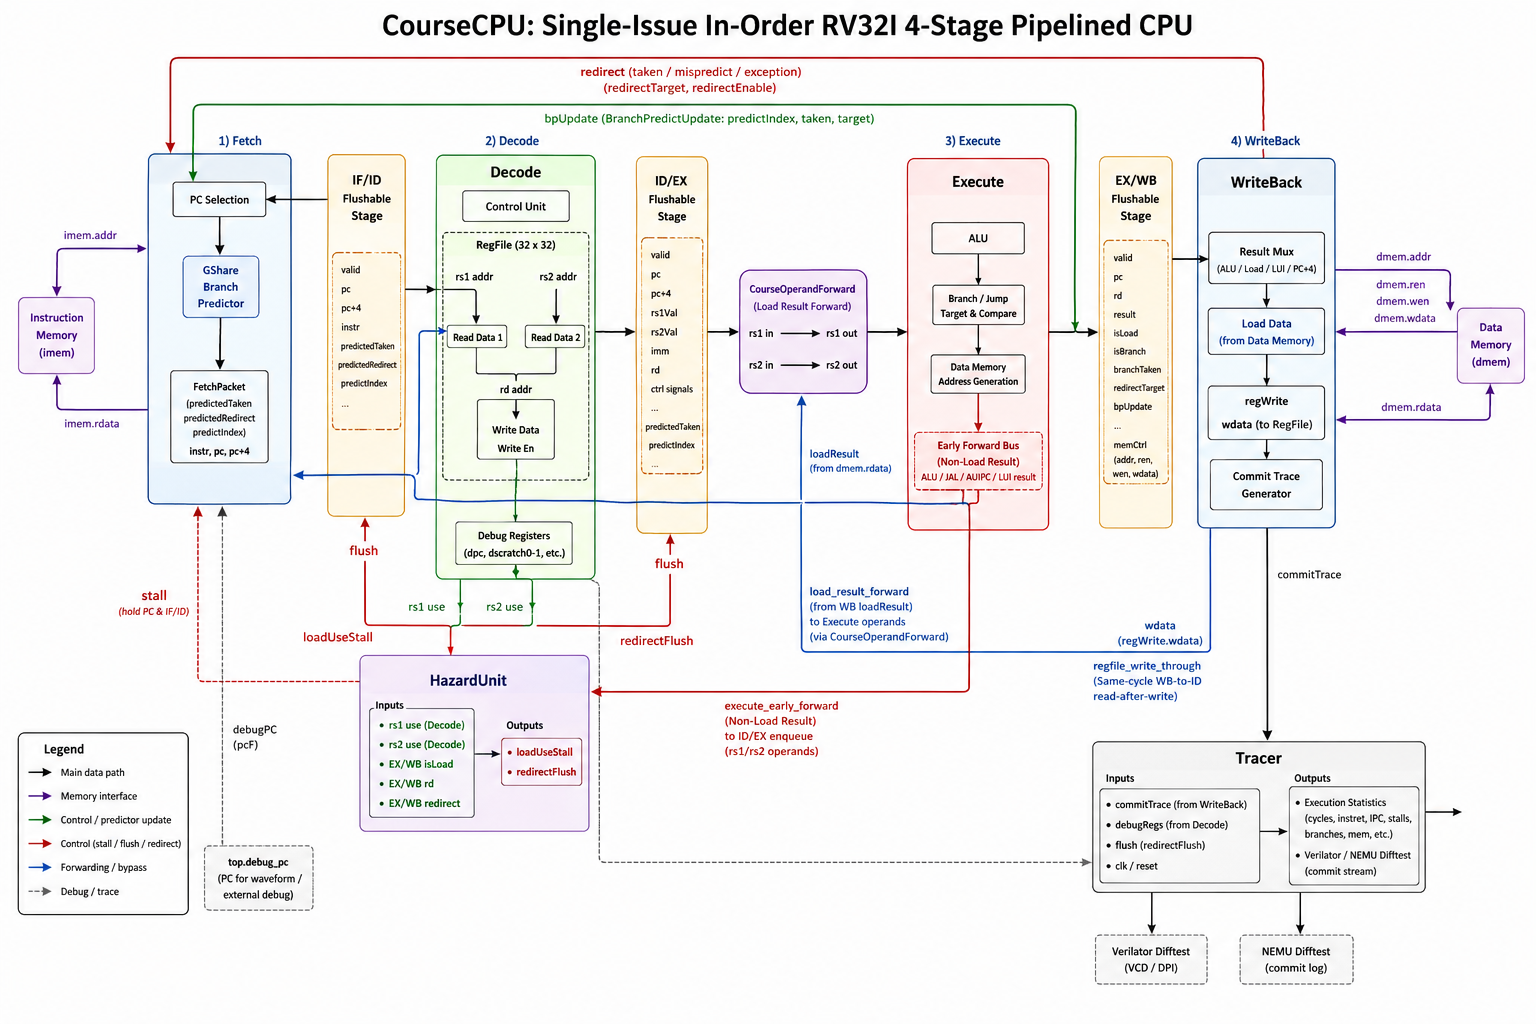
\includegraphics[width=0.95\textwidth]{report_assets/overview_arch.png}
  \caption{CourseCPU 整体架构图}
  \label{fig:overview-arch}
\end{figure}

\chapter{总体设计}

\section{设计目标}

CourseCPU 的总体目标是在保持结构清晰、可综合、可验证的前提下，实现一个能够运行真实 RV32I 程序的四级流水线处理器。设计目标包括：

\begin{itemize}
  \item \textbf{功能完整性：} 实现 RV32I 整数指令级功能，使处理器能够运行由 RISC-V GCC 编译得到的真实 ELF 程序。
  \item \textbf{流水线化：} 使用四级流水线提升吞吐率，并通过 forwarding、stall 和 flush 机制保证流水线正确性。
  \item \textbf{验证可信度：} 建立 Verilator + NEMU difftest 的自动化验证流程，避免只依赖少量手写波形或最终结果检查。
  \item \textbf{FPGA 可实现性：} 生成 Vivado 可综合的 SystemVerilog，并在 FPGA timing、area 和 power 维度进行分析。
  \item \textbf{可配置性：} 对仿真、trace、CSR/SYS、sim ebreak 等功能进行配置化管理，使同一套代码能够服务于仿真、验证和综合。
\end{itemize}

\section{支持的 ISA}

CourseCPU 面向 RV32I 整数指令集。指令类型覆盖了处理器运行真实 C 程序所需的基本能力，包括：

\begin{table}[htbp]
  \centering
  \caption{CourseCPU 支持的主要指令类型}
  \begin{tabularx}{\textwidth}{>{\bfseries}lX}
    \toprule
    指令类型 & 说明 \\
    \midrule
    算术逻辑 & ADD、SUB、AND、OR、XOR、ADDI、ANDI、ORI、XORI 等 \\
    移位 & SLL、SRL、SRA、SLLI、SRLI、SRAI \\
    比较 & SLT、SLTU、SLTI、SLTIU \\
    分支 & BEQ、BNE、BLT、BGE、BLTU、BGEU \\
    跳转 & JAL、JALR \\
    访存 & LB、LH、LW、LBU、LHU、SB、SH、SW，并在实现中保留 byte-addressed memory 语义 \\
    地址生成 & LUI、AUIPC \\
    \bottomrule
  \end{tabularx}
\end{table}

Course 配置下，CPU 面向课程 core 的要求裁剪 CSR/SYS 相关逻辑。这样可以减少无关控制路径和状态寄存器对面积与时序的影响。另一方面，仿真环境中保留 \texttt{sim ebreak} 机制，用于真实程序运行结束时通知仿真框架退出。这一设计将“课程要求的硬件功能”和“仿真平台所需的运行时接口”进行了分离。

\section{单发射顺序执行模型}

CourseCPU 采用 single-issue in-order execution model。处理器每周期最多取指一条、译码一条、执行一条，并在 MEM/WB 阶段最多提交一条指令。所有指令按照程序顺序进入流水线，提交顺序也与程序顺序一致。

这一执行模型具有两个优点。首先，它使流水线行为清晰可解释，便于定位数据冒险、控制冒险和访存错误。其次，它与 NEMU difftest 的 commit 粒度天然匹配：每当 CourseCPU 有一条指令退休，就可以将该指令对应的架构状态与 NEMU 参考模型进行一次对拍。

\section{四级流水线结构}

CourseCPU 采用四级流水线：

\begin{table}[htbp]
  \centering
  \caption{CourseCPU 四级流水线}
  \begin{tabularx}{\textwidth}{>{\bfseries}lX}
    \toprule
    阶段 & 功能 \\
    \midrule
    IF & 维护 PC，访问指令存储器，进行 Fetch 级分支预测，生成 FetchPacket \\
    ID & 译码，读取寄存器堆，生成立即数，生成控制信号和 DecodePacket \\
    EX & 执行 ALU 操作，解析分支条件，生成访存地址、store 数据和 redirect 信息 \\
    MEM/WB & 访问数据存储器，完成 load 数据扩展与寄存器写回，生成 commit trace \\
    \bottomrule
  \end{tabularx}
\end{table}

流水线级间通过 \texttt{FlushableStage} 连接。该模块内部包含 payload register 和 valid register，能够在普通流动、backpressure 和 flush 三种情况下维护流水线状态。CourseCPU 使用 IF/ID、ID/EX 和 EX/WB 三组流水线寄存器，将组合逻辑分布在四个阶段中。

\begin{figure}[htbp]
  \centering
  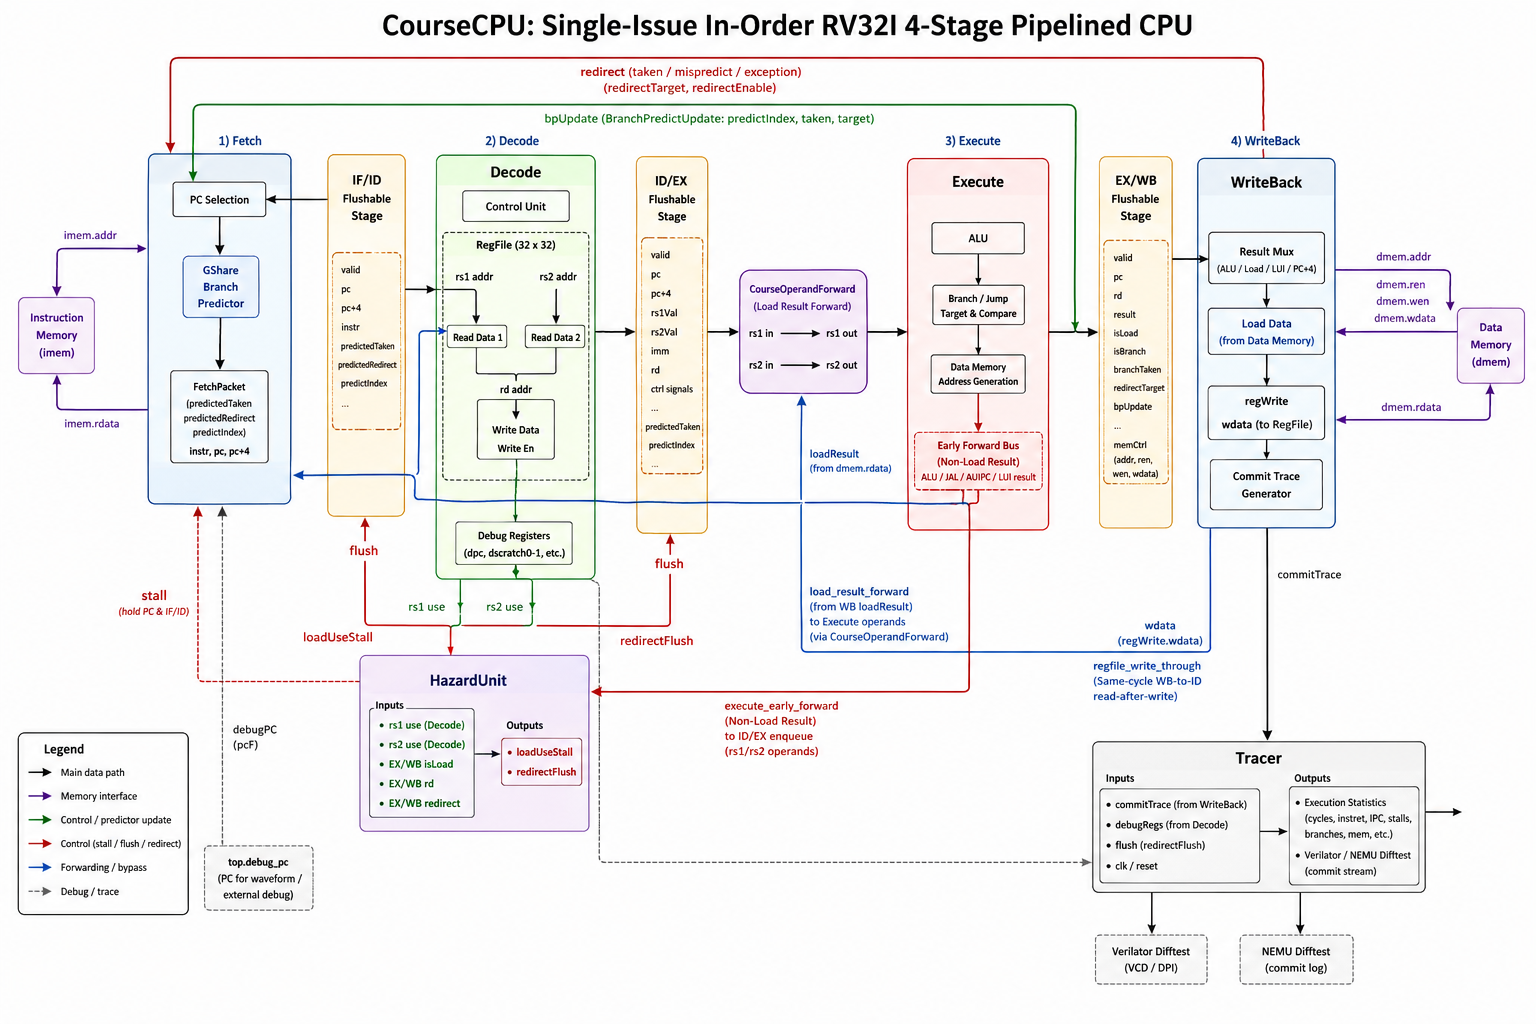
\includegraphics[width=0.95\textwidth]{report_assets/overview_arch.png}
  \caption{CourseCPU 四级流水线与验证接口结构}
  \label{fig:pipeline-arch}
\end{figure}

\section{顶层系统组成}

CourseCPU 顶层由 \texttt{CourseCore} 组织，主要模块包括：

\begin{itemize}
  \item \texttt{Fetch}：负责 PC 维护、指令访问、Fetch 级分支预测和预测目标计算。
  \item \texttt{Decode}：负责指令译码、寄存器堆访问、立即数生成和控制信号生成。
  \item \texttt{CourseOperandForward}：负责对进入 Execute 前的操作数进行 load result forwarding。
  \item \texttt{Execute}：负责 ALU、branch condition、JAL/JALR、访存地址和 redirect 生成。
  \item \texttt{WriteBack}：负责 load 数据处理、寄存器写回和 commit trace 输出。
  \item \texttt{HazardUnit}：负责 load-use stall 和 redirect flush 控制。
  \item \texttt{Tracer}：负责仿真统计、commit trace 和 DPI 调试接口。
\end{itemize}

顶层同时暴露 IMEM、DMEM、debug register、debug PC、retire trace 等接口，使同一个 CPU core 可以被 Verilator 仿真框架、Vivado testbench 和综合顶层复用。

\section{Course 配置与仿真配置}

CourseCPU 采用可配置参数管理调试与仿真功能。例如：

\begin{itemize}
  \item \texttt{enableTraceFields} 控制是否在流水线 packet 中保留 trace 相关字段。
  \item \texttt{enableTracer} 控制是否实例化 tracer。
  \item \texttt{enableDpi} 控制是否启用 DPI 侧的仿真交互。
  \item \texttt{enableSys} 控制是否启用 CSR/SYS 相关译码与执行逻辑。
  \item \texttt{enableSimEbreak} 控制是否保留仿真退出指令路径。
\end{itemize}

这种配置化方式使 CourseCPU 能够在“用于课程提交的精简综合配置”和“用于仿真调试的完整 trace 配置”之间切换。最终 Course 配置中，CSR/SYS 被裁剪以优化面积和时序，而 sim ebreak 被保留以服务真实程序仿真。

\chapter{微架构设计}

\section{流水线整体组织}

CourseCPU 的流水线组织围绕 packet 传递展开。IF 阶段输出 \texttt{FetchPacket}，ID 阶段输出 \texttt{DecodePacket}，EX 阶段输出 \texttt{ExecutePacket}。这些 packet 通过 \texttt{FlushableStage} 保存，使各级之间既能传递数据，也能传递控制信号、预测信息和 trace 信息。

流水线采用 valid/ready 风格的握手控制。当前级只有在下一级 ready 时才会推进；当发生 redirect flush 时，对应流水线寄存器的 valid 位被清空，错误路径指令不会继续向后提交。与简单的全局 enable 流水线相比，这种组织方式更接近现代硬件设计中常用的 decoupled pipeline 风格，也更便于处理 stall、flush 和 backpressure 的组合情况。

\section{IF 阶段：取指与 PC 选择}

IF 阶段由 \texttt{Fetch} 模块实现。它维护 \texttt{pcReg}，向 IMEM 输出取指地址，并从 IMEM 接收 32-bit instruction。默认情况下，下一条 PC 为 \texttt{pc + 4}。当后端产生 redirect 时，redirect target 具有最高优先级，PC 被更新为正确目标地址。

CourseCPU 在 IF 阶段集成了轻量级 GShare Branch Predictor。Fetch 使用当前 PC 查询 predictor，并对 branch/JAL 指令在取指级计算预测目标。对于 conditional branch，如果预测为 taken，则下一条 PC 选择 branch target；对于 JAL，Fetch 可直接预测 redirect；JALR 依赖寄存器值，仍需在 EX 阶段解析。

IF 阶段输出的 \texttt{FetchPacket} 不仅包含 PC 和 instruction，也包含预测相关字段，例如 predicted taken、predicted redirect 和 predictor index。这些信息随流水线向后传递，在 EX 阶段用于判断预测是否正确，并反馈更新 predictor。

\section{ID 阶段：译码、寄存器读取、立即数生成}

ID 阶段由 \texttt{Decode} 模块实现，主要任务包括：

\begin{itemize}
  \item 解析 opcode、funct3、funct7、rs1、rs2、rd 等字段。
  \item 生成 ALU 操作类型、branch 类型、memory 操作类型和 writeback 控制信号。
  \item 从寄存器堆读取 rs1 和 rs2。
  \item 生成 I/S/B/U/J 等立即数。
  \item 生成 hazard detection 所需的 rs1/rs2 使用信息。
\end{itemize}

寄存器堆采用 32 个 32-bit 通用寄存器，其中 x0 固定为 0。写回来自 MEM/WB 阶段。为了保证同周期读写同一寄存器时读取到最新值，寄存器堆包含 write-through 行为：当读地址与当前写回地址相同且写使能有效时，读端直接返回写回数据。

ID 阶段还负责将 Fetch 阶段预测信息转化为后续流水线可理解的 branch prediction bundle。对于已在 Fetch 级完成 redirect 的预测，Decode 会记录该预测状态；对于 JAL 等能够在 Decode 侧确认的直接跳转，也会携带预测 redirect 信息。这些信息用于后续 EX 阶段判断是否需要恢复 PC。

\section{EX 阶段：ALU、分支解析与访存地址生成}

EX 阶段由 \texttt{Execute} 模块实现，是 CourseCPU 的主要计算阶段。其输入来自 ID/EX 流水线寄存器，并经过 operand forwarding 后进入执行逻辑。

EX 阶段完成以下操作：

\begin{itemize}
  \item 对 ADD、SUB、AND、OR、XOR、shift、SLT 等指令执行 ALU 运算。
  \item 对 branch 指令计算条件结果，例如 equal、not equal、less than、greater or equal。
  \item 对 JAL/JALR 生成跳转目标。
  \item 对 load/store 生成 byte-addressed memory address。
  \item 对 control flow 指令生成 redirect 信息。
  \item 生成写回数据或访存请求，并输出 \texttt{ExecutePacket}。
\end{itemize}

分支的最终正确性在 EX 阶段确定。如果 Fetch/Decode 携带的预测结果与 EX 阶段真实结果不一致，EX 生成 redirect，顶层控制逻辑随后 flush 错误路径的 IF/ID 和 ID/EX 指令，并将 Fetch PC 更新到正确目标。

\section{MEM/WB 阶段：访存与写回}

CourseCPU 将 MEM 与 WB 合并为一个阶段。EX/WB 流水线寄存器保存来自 Execute 的结果，WriteBack 模块根据 memory control 信号判断当前指令是否为 load、store 或普通 ALU/writeback 指令。

对于普通 ALU 指令，WriteBack 直接将 EX 结果写回寄存器堆。对于 load 指令，WriteBack 从 DMEM 接收读数据，并根据访存类型进行字节或字数据选择与符号扩展。对于 store 指令，CourseCore 顶层将地址、写使能和写数据输出到 DMEM 接口。

MEM/WB 阶段也是 CourseCPU 的 commit 点。只有到达该阶段且有效的指令才会产生 retire trace。该设计使 Verilator + NEMU difftest 可以以 commit 为单位比较架构状态，保证错误路径指令不会污染 reference model。

\section{流水线寄存器与 valid/ready 控制}

\texttt{FlushableStage} 是 CourseCPU 的通用流水线寄存器模块。它由 payload register 和 valid register 组成：

\begin{itemize}
  \item payload register 保存 packet 数据。
  \item valid register 表示当前流水线槽是否包含有效指令。
  \item 当 enq fire 时写入新 payload 并置 valid。
  \item 当 deq fire 且没有新指令进入时清除 valid。
  \item 当 flush 有效时清除 valid，使错误路径指令失效。
\end{itemize}

这种设计使 flush 不需要修改 packet 中每一个字段，只需要清除 valid 即可阻止错误路径指令继续提交。同时，valid/ready 握手也使 load-use stall 和后端 backpressure 可以自然地阻塞前级。

\section{Byte-addressed Memory Interface}

CourseCPU 的 IMEM 和 DMEM 均使用 byte address。IMEM 接口中，Fetch 输出当前 PC 作为 instruction address，IMEM 返回对应的 32-bit instruction。DMEM 接口中，Execute 生成 byte address，WriteBack/顶层根据 memory control 信号完成 load/store。

对于 \texttt{LW/SW}，地址表示字节地址，但访问粒度为 32-bit word。对于 \texttt{LB/SB}，地址同样为字节地址，低地址位用于选择目标 byte。LB 需要根据 signed/unsigned 属性进行符号扩展或零扩展；SB 只写入低 8 位数据到目标 byte lane。

这种 byte-addressed memory interface 与真实 RISC-V 软件环境一致，也使 ELF loader 能够按照程序段中的真实地址布局装载 text/data。

\chapter{冒险处理机制}

\section{RAW 数据相关模型}

CourseCPU 是单发射顺序流水线，指令按顺序进入流水线，但不同指令在不同流水级中并行执行，因此仍然存在 RAW 数据相关。例如后一条指令在 ID/EX 或 EX 阶段需要读取某个寄存器，而前一条指令的结果尚未写回寄存器堆。

典型 RAW 场景包括：

\begin{itemize}
  \item ALU-to-ALU：前一条 ALU 指令产生的结果被后一条 ALU 指令立即使用。
  \item ALU-to-branch：前一条指令产生的结果被后一条 branch 用作比较操作数。
  \item load-to-use：load 指令从数据存储器读取的结果被紧随其后的指令使用。
  \item writeback-to-decode：MEM/WB 阶段写回寄存器的同周期，Decode 阶段读取同一寄存器。
\end{itemize}

CourseCPU 使用 forwarding、寄存器堆 write-through 和 load-use stall 共同处理这些相关。

\section{两级 Forwarding 网络}

CourseCPU 的 forwarding 逻辑分为两类。第一类是 execute result early forwarding。当 Execute 阶段已经产生非 load 指令的结果，且该结果会写回寄存器时，如果当前 Decode 输出指令的 rs1 或 rs2 等于该 rd，则在写入 ID/EX 流水线寄存器前直接用 execute result 覆盖对应 operand。该路径用于缩短常见 ALU-to-ALU RAW 的等待时间。

第二类是 load result forwarding。由于 load 数据在 MEM/WB 阶段才可用，CourseCPU 在 \texttt{CourseOperandForward} 中接收 WriteBack 输出的 memory packet，并在进入 Execute 前对 rs1/rs2 进行选择。如果 forwarding valid 且目标寄存器匹配，则使用 load result 替代 Decode 阶段读取到的旧值。

所有 forwarding 均忽略 x0，因为 RISC-V 规定 x0 恒为 0，任何对 x0 的写入都不应影响后续读取。

\section{Load-use 冒险检测与停顿}

load-use 冒险是指 load 指令之后紧跟使用其结果的指令。即使数据存储器在仿真模型中看起来是低延迟的，从流水线时序角度看，load result 仍然在 MEM/WB 阶段才成为可写回/可转发的数据。如果后一条指令不等待一个周期，就可能在 Execute 阶段使用到旧值。

CourseCPU 使用 HazardUnit 检测 load-use 场景。当 Decode 阶段指令使用的 rs1/rs2 与后续 load 的 rd 冲突时，HazardUnit 产生 load-use stall。stall 会阻止 Fetch 和 Decode 继续推进，使 load 指令先进入可转发阶段。停顿之后，后一条指令通过 forwarding 网络获得正确 load result。

在当前 CourseCPU 中，经过多轮优化后，load forwarding 与 execute early forwarding 被区分处理，避免将不必要的写回路径拉回 Decode 侧造成更差的 routing critical path。

\section{控制冒险处理}

控制冒险来自 branch、JAL 和 JALR 等改变 PC 的指令。CourseCPU 支持 Fetch 级预测，但最终控制流正确性仍在 EX 阶段确认。EX 阶段会根据真实 branch condition 或 jump target 判断当前预测是否正确。

当预测正确时，流水线继续执行，不需要额外恢复。当预测错误时，EX/WB 侧产生 redirect 信息，顶层将 Fetch PC 更新为正确目标，并 flush IF/ID 和 ID/EX 中的错误路径指令。这样可以保证错误路径指令不会进入 commit 点，也不会影响寄存器堆和数据存储器的架构状态。

\section{Redirect 与 Flush 机制}

CourseCPU 的 redirect 机制包含 valid 和 target 两部分。redirect valid 表示当前周期需要修正 PC，redirect target 表示正确的下一条取指地址。redirect 来源主要包括：

\begin{itemize}
  \item EX 阶段发现 branch prediction 错误。
  \item JAL/JALR 产生跳转目标。
  \item Decode/Fetch 协作预测路径需要进行前端 redirect。
\end{itemize}

flush 作用于流水线寄存器的 valid 位。发生 redirect flush 时，IF/ID 与 ID/EX 中的错误路径指令被清空。由于 CourseCPU 的 commit 点在 MEM/WB 阶段，且 flush 会阻止错误路径继续向后推进，因此 commit trace 与 NEMU difftest 的对拍只会看到架构上真实提交的指令。

\section{Flush、Stall 与 Forwarding 的优先级关系}

CourseCPU 中 flush、stall 和 forwarding 分别处理不同层次的问题：

\begin{itemize}
  \item flush 处理控制流错误，是改变流水线有效性的控制信号。
  \item stall 处理数据尚未可用的情况，是暂停流水线推进的控制信号。
  \item forwarding 处理数据值选择，不改变指令是否有效，也不改变流水线控制流。
\end{itemize}

当 redirect flush 发生时，它优先清除错误路径指令。load-use stall 则保持前端和 Decode 侧不继续推进，等待数据进入可转发阶段。forwarding 在指令仍然有效且准备进入 Execute 时修正 operand value。通过这种优先级划分，CourseCPU 能够同时处理数据冒险和控制冒险，而不会让错误路径指令或旧 operand 污染最终提交状态。

\chapter{分支预测机制}

\section{分支预测的设计动机}

在四级流水线中，控制流指令会直接影响前端取指方向。若采用最简单的静态预测策略，即所有条件分支默认预测为 not taken，则当真实程序中存在循环、条件判断和函数调用时，前端会频繁取到错误路径指令。错误路径指令虽然会被 EX 阶段 redirect flush 清除，但这些周期无法产生有效提交，从而降低 IPC。

真实 C 程序中的分支密度通常高于人工 directed test。以 \texttt{quick-sort} 这类程序为例，递归调用、数组划分、循环比较都会产生大量条件分支。如果每次 taken branch 都等待 EX 阶段解析后再 redirect，流水线前端将持续付出 flush penalty。因此 CourseCPU 在保持 EX 阶段最终解析语义不变的前提下，在 Fetch 阶段加入轻量级分支预测机制。

\section{Fetch 级 GShare Branch Predictor}

CourseCPU 的分支预测器位于 Fetch 阶段。Fetch 使用当前 \texttt{pcReg} 查询 GShare predictor，得到方向预测结果和预测表 index。GShare predictor 使用 PC 信息与 global history 组合生成索引，使不同分支在预测表中的访问能够部分携带全局控制流历史。

CourseCPU 的实现中，predictor entries 当前配置为 8。这个大小是面积和性能之间的折中：entries 过多会增加 LUT/FF 和 routing 压力，entries 过少则会导致不同分支之间 aliasing 增强。实验过程中曾尝试更复杂的 BTB 方案，但由于面积和实现复杂度增加明显，最终采用更轻量的 Fetch 级方向预测和目标计算方案。

\section{预测目标计算}

Fetch 阶段直接从当前 instruction 中解析 opcode，并识别 branch 和 JAL 指令。对于 branch 指令，Fetch 计算 B-type immediate；对于 JAL，Fetch 计算 J-type immediate。若 branch 被预测为 taken，或者指令为 JAL，则 Fetch 将下一条 PC 选择为当前 PC 加对应立即数；否则 PC 按顺序更新为 \texttt{pc + 4}。

JALR 的目标依赖 rs1 寄存器值，因此无法在 Fetch 阶段仅根据指令编码得到完整目标地址。CourseCPU 对 JALR 保持 EX 阶段解析，避免将寄存器读取或复杂 forwarding 逻辑拉入前端关键路径。

\section{Predictor 更新与错误恢复}

预测信息随 FetchPacket 向后传递。EX 阶段得到真实 branch result 后，会判断预测结果是否与实际控制流一致。若预测错误，EX/WB 侧产生 redirect，顶层控制逻辑 flush IF/ID 和 ID/EX 中的错误路径指令，并将 Fetch PC 修正为正确目标。

predictor 的更新在指令到达后端并确认真实结果后进行。这样可以避免错误路径上的指令污染预测器状态。更新信息包括 predictor index、预测方向和真实 taken 信息。由于 CourseCPU 是顺序提交处理器，预测器更新顺序与程序顺序保持一致，简化了实现和验证。

\section{IPC 与 Flush Probability}

CourseCPU 在仿真框架中统计总周期数、提交指令数和 flush 次数，并计算 IPC 与 flush probability。该统计直接反映分支预测和控制冒险恢复机制对真实程序性能的影响。

在优化过程中，CourseCPU 曾从约 0.75 IPC 提升到约 0.84 IPC。提升主要来自 Fetch 级分支预测减少错误路径取指和 flush penalty。虽然该 predictor 仍然较轻量，但它在面积开销较小的前提下获得了可观的真实性能收益。

\begin{table}[htbp]
  \centering
  \caption{最终版本真实程序性能统计}
  \begin{tabular}{lrrrr}
    \toprule
    程序 & Cycles & Instructions & IPC & Flush Probability \\
    \midrule
    add-longlong & 1889 & 1640 & 0.868184 & 0.050000 \\
    bubble-sort & 3792 & 3156 & 0.832278 & 0.066857 \\
    quick-sort & 3904 & 3304 & 0.846311 & 0.060230 \\
    recursion & 9172 & 6550 & 0.714130 & 0.133282 \\
    select-sort & 4126 & 3655 & 0.885846 & 0.042681 \\
    \midrule
    加权汇总 & 22883 & 18305 & 0.799939 & 0.083092 \\
    \bottomrule
  \end{tabular}
\end{table}

从表中可见，当前最终版本在五个真实 C benchmark 上加权 IPC 为 0.799939。若不按指令数加权，而是对各 benchmark IPC 直接取算术平均，则平均 IPC 为 0.829350。recursion 程序包含间接函数调用、递归返回和除法 helper 例程，控制流更复杂，因此 flush probability 达到 13.3282\%，是拉低整体加权 IPC 的主要样本。select-sort 的分支行为更规律，IPC 最高，为 0.885846。

\chapter{仿真与验证平台}

\section{Verilator 周期级仿真框架}

CourseCPU 使用 Chisel 描述硬件，并生成 SystemVerilog RTL。仿真环境使用 Verilator 将 RTL 编译为 C++ cycle model，再由 C++ 仿真框架驱动时钟、复位、存储器接口和外部调试接口。

Verilator 仿真框架相比传统 Verilog testbench 具有更强的工程可扩展性。它能够方便地接入 ELF loader、NEMU difftest、反汇编、trace、性能统计和命令行参数，并支持运行较大规模的真实程序。对于 CPU 设计而言，这类 cycle-level simulator 更接近真实处理器开发中的仿真验证环境。

在运行时，Verilator 仿真器并不只是简单地“跑若干周期”。它维护统一的仿真上下文，负责解析命令行参数、加载 ELF、初始化内存、驱动 CPU 时钟、接收 commit trace、调用 difftest、记录 flush 事件，并在程序通过 \texttt{ebreak} 退出后输出执行统计。CPU RTL、仿真内存、DPI 接口和 reference model 通过这一 C++ 仿真框架形成完整闭环。

从工程组织上看，仿真平台分为三个层次。最底层是 Verilator 生成的 cycle model，负责提供可执行的 RTL 行为模型；中间层是 C++ simulation runtime，负责时钟推进、复位、内存访问、DPI bridge、trace 和统计；最上层是程序运行与调试接口，包括 ELF loader、SDB、difftest 和性能报告。这样的分层使硬件 RTL 可以保持清晰，而仿真平台能够承载真实软件运行所需的复杂基础设施。

与传统 testbench 相比，这一平台的优势是“同一份 RTL 面向不同验证深度复用”。快速 directed case 可以通过 Scala/Chisel test 或 RTL readmemh testbench 检查，真实程序则通过 Verilator + ELF loader 执行，出现错误时再通过 difftest、SDB、trace 和 waveform 逐层定位。这种调试路径避免了只靠波形从海量信号里盲找问题。

\section{交互式 SDB 调试器}

仿真平台保留了类似 NEMU 的交互式 SDB 调试能力。SDB 提供单步执行、连续运行、查看寄存器、查看内存、反汇编当前 PC 附近指令等调试入口。与纯波形调试相比，SDB 更适合定位架构级错误：当 difftest 报出某条指令后状态不一致时，可以通过 SDB 回到对应 PC、查看通用寄存器和内存，再结合 commit trace 判断错误来自译码、执行、访存还是写回。

这种交互式调试能力对流水线 CPU 尤其重要。波形能够展示微架构信号如何变化，但 SDB 能直接展示软件视角下的架构状态。二者结合后，调试流程可以从“difftest 精确报错”出发，经由 SDB 定位出错指令和状态，再进入 GTKWave/Vivado waveform 查看该指令在流水线中的传播过程。

\begin{figure}[H]
  \centering
  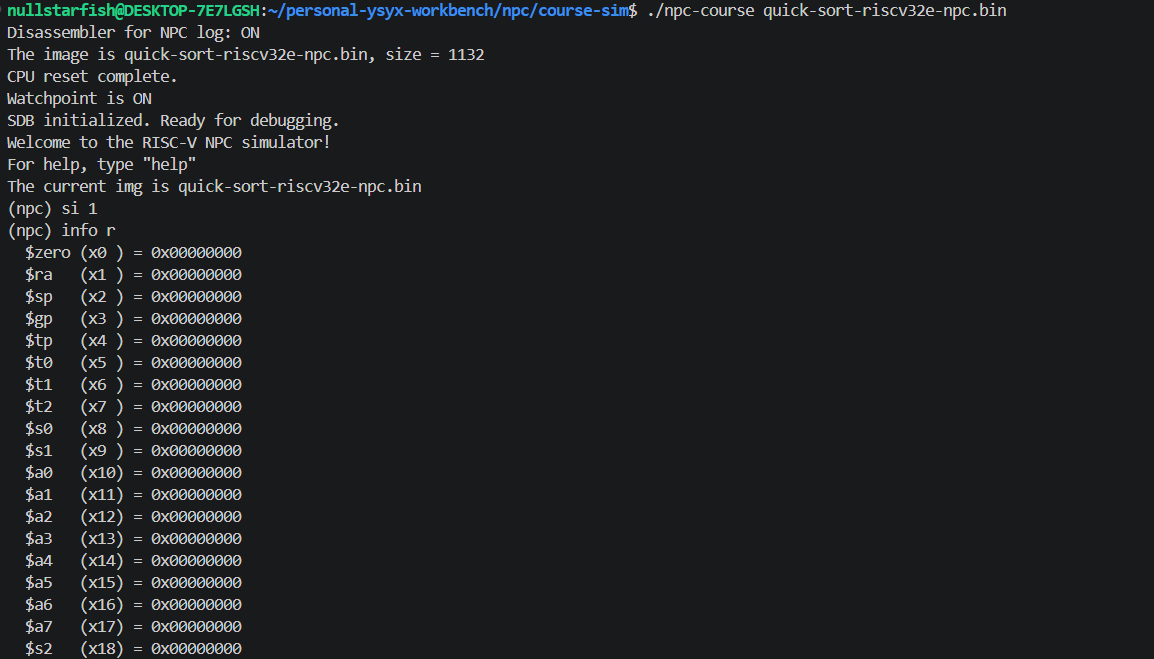
\includegraphics[width=0.95\textwidth]{report_assets/sdb_peek.png}
  \caption{CourseCPU Verilator 仿真平台中的交互式 SDB 调试界面}
  \label{fig:sdb-peek}
\end{figure}

\begin{table}[H]
  \centering
  \caption{SDB 支持的主要交互式命令}
  \begin{tabularx}{\textwidth}{lX}
    \toprule
    命令 & 功能 \\
    \midrule
    \texttt{help} & 打印所有支持的调试命令，或查看指定命令说明。 \\
    \texttt{c} & 连续运行程序，直到程序结束、触发 watchpoint 或出现错误。 \\
    \texttt{q} & 退出仿真器。 \\
    \texttt{si [N]} & 单步执行 N 条指令，未指定 N 时默认执行一条。 \\
    \texttt{info r} & 打印当前 CPU 通用寄存器与 PC 等架构状态。 \\
    \texttt{info w} & 打印当前 watchpoint 列表。 \\
    \texttt{x N EXPR} & 从表达式给出的地址开始扫描 N 个 word 的内存内容。 \\
    \texttt{p EXPR} & 求值表达式，可用于查看寄存器、立即数和地址计算结果。 \\
    \texttt{w EXPR} & 添加 watchpoint，当表达式值变化时暂停执行。 \\
    \texttt{d N} & 删除编号为 N 的 watchpoint。 \\
    \bottomrule
  \end{tabularx}
\end{table}

\section{RISC-V GCC 编译流程}

CourseCPU 的测试程序不是只通过手写机器码或固定 \texttt{.mem} 文件构造，而是使用真实 RISC-V GCC 工具链从 C/汇编源码编译生成 ELF 文件。当前环境中使用的交叉编译器为 \texttt{riscv64-linux-gnu-gcc (Debian 14.2.0-19) 14.2.0}。在 Abstract-Machine 的 \texttt{riscv32e-npc} 目标中，构建参数进一步覆盖为 \texttt{-march=rv32e\_zicsr -mabi=ilp32e}，并生成 \texttt{elf32-littleriscv} 格式程序镜像。该流程覆盖了编译器、链接器、ABI、函数调用、栈布局、全局数据段等真实软件环境因素。

这意味着 CourseCPU 需要正确支持真实程序运行所需的控制流、访存、寄存器约定和程序布局，而不只是执行几条孤立指令。当前 performance 测试集中包含 \texttt{add-longlong}、\texttt{bubble-sort}、\texttt{quick-sort}、\texttt{recursion} 和 \texttt{select-sort}。这些程序覆盖 64-bit 软件整数运算、数组访存、排序循环、递归调用、函数指针间接调用、除法 helper 例程和多种分支模式，说明处理器、仿真平台和软件工具链之间已经形成完整闭环。

\section{ELF Loader 与程序装载}

仿真框架包含 ELF loader。运行程序前，loader 解析 ELF 文件中的 program header，将 text/data 等 segment 按 ELF 中记录的物理地址装载到仿真内存空间中，并设置程序入口地址。这样，CourseCPU 在仿真中看到的指令和数据布局与真实链接结果一致。

ELF 装载比简单 \texttt{readmemh} 更接近真实系统执行环境。一方面，它支持程序段和数据段分离；另一方面，它避免了手工维护指令地址与数据地址带来的错误。对于需要运行真实 C 程序的 CPU 项目而言，ELF loader 是验证平台的重要组成部分。

\section{Abstract-Machine C SDK}

CourseCPU 使用基于 \texttt{abstract-machine} 的 C source SDK 构建测试程序。该 SDK 为裸机程序提供统一的运行入口、链接脚本、基础运行时和退出机制，使测试程序可以用接近普通 C 程序开发的方式编写。

这种方式显著提高了测试程序的表达能力。开发者可以编写排序、数学计算、字符串处理等真实程序，而不需要手工展开为汇编或机器码。这也使 CourseCPU 的验证从“指令能不能执行”提升到“处理器能不能承载真实软件负载”的层次。

Abstract-Machine 在本项目中的价值主要体现在四点。第一，它提供统一的 \texttt{\_start} 和 \texttt{\_trm\_init} 启动路径：\texttt{\_start} 设置栈指针并跳转到 \texttt{\_trm\_init}，随后由 \texttt{\_trm\_init} 调用用户 \texttt{main()} 并在结束时通过 \texttt{halt/ebreak} 通知仿真框架退出。第二，它通过完整链接脚本定义 \texttt{ENTRY(\_start)}、text/data/bss 段、\texttt{\_stack\_pointer}、\texttt{\_heap\_start} 等符号，使 ELF loader 可以按真实地址装载 text/data 并为裸机 C 程序提供栈与堆空间。第三，它提供 \texttt{ioe\_init()} 等外设初始化入口，当前 NPC 平台注册 timer、RTC、UART/input 等 AM 设备抽象，使程序可以通过统一 AM API 访问仿真外设。第四，它将 \texttt{check()} 与 \texttt{halt/ebreak} 封装为通用测试接口，使 C 程序可以直接表达正确性断言，并在结束时通知仿真框架收集统计数据。

因此，本项目中的 performance benchmark 并不是手工拼出的机器码片段，而是由真实 RISC-V GCC 工具链编译的 C 程序。程序经过 Abstract-Machine 运行时链接后生成 ELF，仿真器按 ELF program header 装载指令和数据段，CPU 再通过正常取指、访存、函数调用和退出路径完成执行。这使 benchmark 的软件栈、程序布局和 ABI 行为更接近真实裸机程序。

\begin{figure}[H]
  \centering
  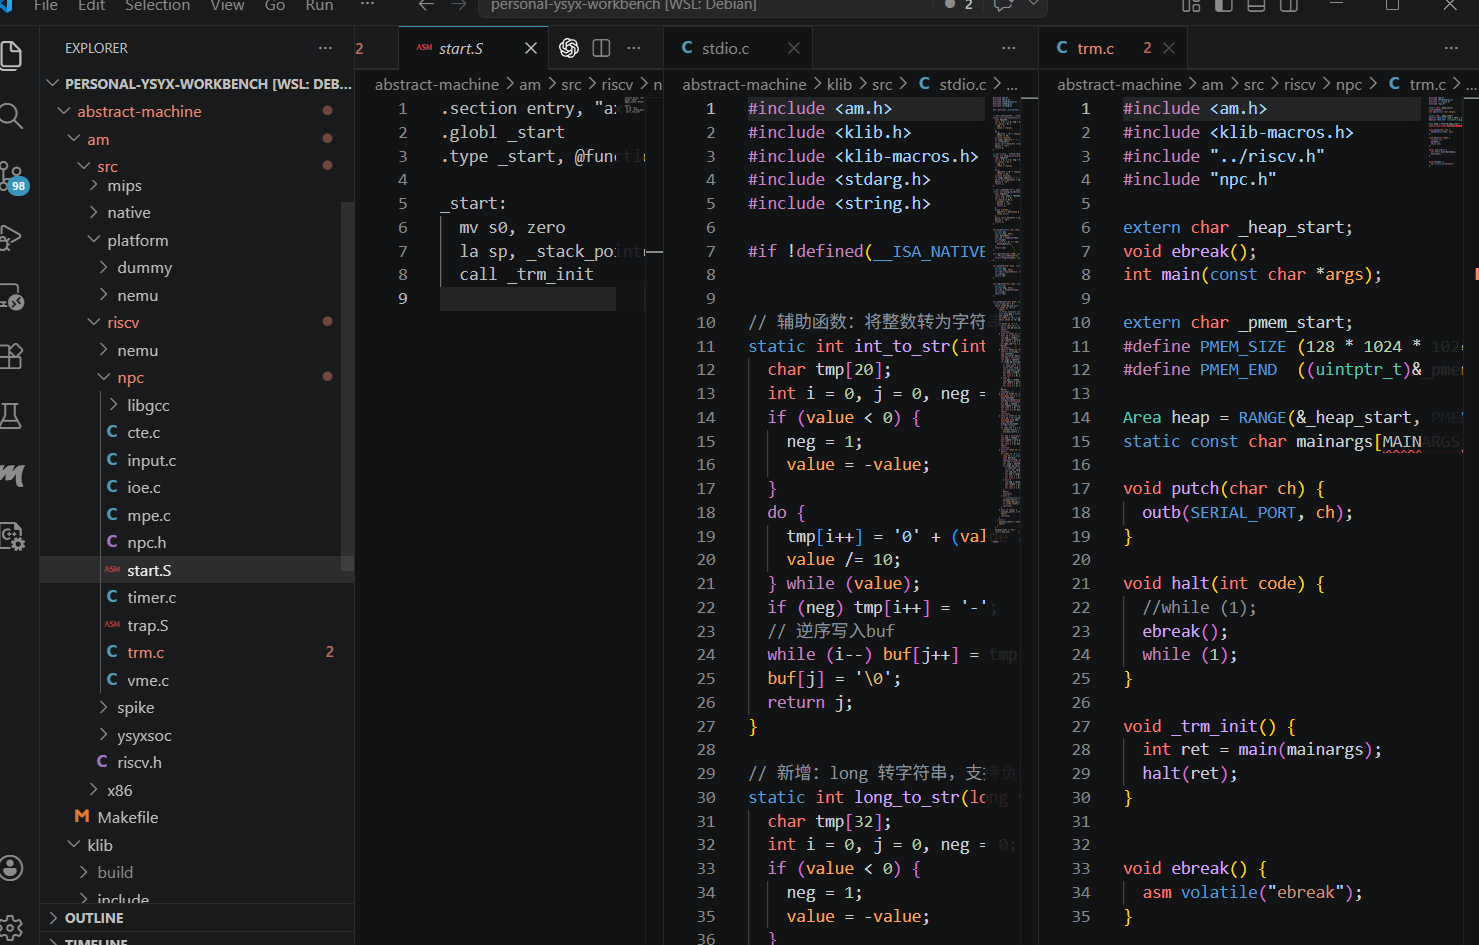
\includegraphics[width=0.95\textwidth]{report_assets/am_peek.png}
  \caption{Abstract-Machine 构建与运行时环境：真实 C 程序经 GCC、链接脚本与 AM runtime 进入 CourseCPU 仿真平台}
  \label{fig:am-peek}
\end{figure}

\section{NEMU Differential Testing}

CourseCPU 接入 NEMU 作为 reference model 进行 Differential Testing。每当 CourseCPU 提交一条指令时，仿真框架将该指令对应的架构状态与 NEMU 执行同一条指令后的状态进行比较。比较内容包括 PC、通用寄存器以及必要的访存副作用。

Difftest 最重要的价值在于它检查的是每一条指令提交后的寄存器状态，而不是程序结束后的单个结果。CourseCPU 在 MEM/WB commit 点导出 DUT 的 PC 和 32 个通用寄存器，NEMU reference model 同步执行一条指令后返回 reference register file，仿真框架逐项比较 \texttt{GPR[0..31]} 与 PC；若任意寄存器或 PC 不一致，仿真会立即停止并打印 DUT/ref 两侧寄存器快照。若流水线 forwarding、load 扩展、branch flush 或写回控制存在错误，difftest 往往能在错误第一次污染架构状态时定位到具体提交指令。这比只检查最终内存地址的 testbench 更严格，也更适合 CPU 级验证。

在 CourseCPU 中，difftest 的驱动点位于 MEM/WB 提交阶段。只有 retire valid 的指令才会送入 reference model，对错误路径被 flush 的指令不会进行对拍。这与处理器架构语义一致：微架构可以取到、译码甚至部分执行错误路径指令，但只要它们不提交，就不应影响 NEMU reference state。该机制能够自然验证 flush 精确性、writeback 正确性和 load/store 副作用。

\begin{figure}[H]
  \centering
  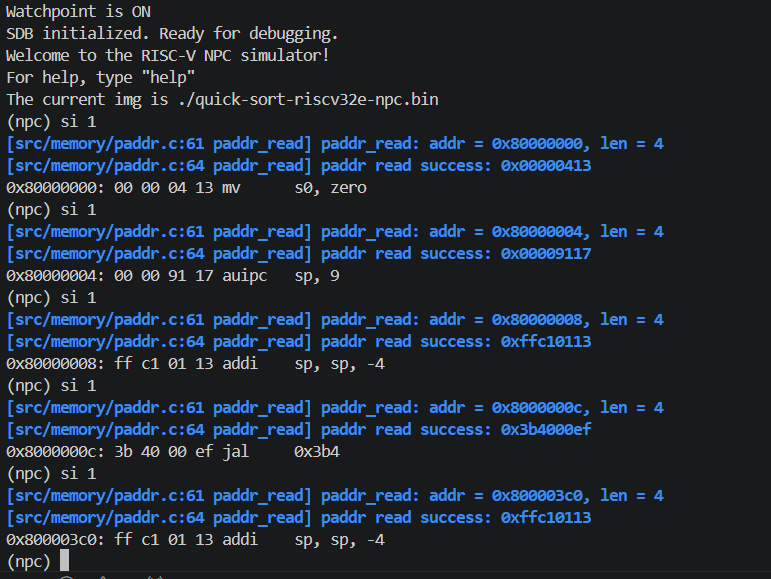
\includegraphics[width=0.95\textwidth]{report_assets/difftest_peek.png}
  \caption{NEMU difftest 对拍：每条提交指令后比较 DUT 与 reference model 的寄存器状态}
  \label{fig:difftest-peek}
\end{figure}

\section{Commit Trace 与统计信息}

CourseCPU 在 MEM/WB 阶段生成 retire trace，包括 retire valid、retire PC、retire instruction 和寄存器状态等信息。仿真框架利用这些信息驱动 difftest，同时统计执行周期数、提交指令数、flush 次数和 IPC。

统计输出示例包括：

\begin{lstlisting}[language={}]
Execution Statistics:
  Total Cycles:       ...
  Total Instructions: ...
  Total Flushes:      ...
  Average IPC:        ...
  Flush Probability:  ...
\end{lstlisting}

这些统计数据使性能分析和微架构优化能够基于真实 workload，而不是只依赖波形观察。

\chapter{Vivado RTL 兼容性验证}

\section{验证目标}

虽然 CourseCPU 的主验证环境是 Verilator + NEMU difftest，但 Vivado RTL 仿真仍然是本项目的重要补充。Vivado 仿真用于证明生成的 SystemVerilog RTL 能够在 FPGA 工具链中直接运行，并验证 IMEM/DMEM 接口、流水线控制信号和关键冒险处理波形符合预期。

因此，Vivado RTL 兼容性验证的定位不是替代 difftest，而是提供面向课程交付和 FPGA 工具流的波形证据。两者互补：Verilator + NEMU 用于大规模功能正确性验证，Vivado waveform 用于展示 RTL 级接口行为和关键时序过程。

\section{RTL 兼容顶层与 \texttt{readmemh} 存储器}

为满足传统 RTL 仿真和课程验收要求，本项目额外提供了 \texttt{CourseCompatibleTop}。该顶层不依赖 DPI 存储器，而是将 \texttt{CourseCore} 连接到纯 RTL 的 \texttt{CompatibleIMem} 与 \texttt{CompatibleDMem}。两者均支持通过 SystemVerilog \texttt{\$readmemh} 从 \texttt{.mem} 文件装载程序或数据。

\begin{itemize}
  \item \texttt{CompatibleIMem} 使用 \texttt{+IMEM=<path>} 指定 instruction memory image。
  \item \texttt{CompatibleDMem} 使用可选 \texttt{+DMEM=<path>} 指定 data memory image，并支持 byte/half/word load-store。
  \item \texttt{tb\_CourseCompatibleTop.sv} 是统一 testbench，通过 \texttt{+TEST=<name>} 选择期望检查，通过 \texttt{+DUMPFILE} 与 \texttt{+WAVE\_START}/\texttt{+WAVE\_END} 导出局部 VCD 波形。
  \item 每个 \texttt{.mem} 文件均配套同名 \texttt{.S} 汇编源文件，保证机器码输入可读、可审查、可复现。
\end{itemize}

这一兼容层的定位是课程/Vivado 风格的波形展示与 RTL 接口验证。它与主线 Verilator + ELF + NEMU difftest 环境共享同一个 CourseCPU RTL，但采用 \texttt{readmemh} 程序镜像和传统 testbench 驱动方式，便于在 GTKWave 或 Vivado waveform 中展示流水线冒险处理。

\section{IMEM 兼容性测试}

IMEM 接口采用 byte address。Fetch 阶段输出 \texttt{imem.addr}，外部指令存储器返回对应的 32-bit instruction。Vivado IMEM 兼容测试应观察以下行为：

\begin{itemize}
  \item 复位后 PC 从 start address 开始取指。
  \item 无 redirect 时，\texttt{imem.addr} 按 \texttt{pc + 4} 顺序递增。
  \item branch/JAL 预测或后端 redirect 后，\texttt{imem.addr} 更新为目标地址。
  \item IF/ID valid 在 flush 时被清空，错误路径指令不会继续后传。
\end{itemize}

报告中建议放置一张“正常取指与 PC 更新”波形，以及一张“redirect 后 PC 修正”波形。

\section{DMEM 兼容性测试}

DMEM 接口同样采用 byte address。顶层输出 \texttt{dmem.addr}、\texttt{dmem.ren}、\texttt{dmem.wen}、\texttt{dmem.wdata}、\texttt{dmem.subop} 和 \texttt{dmem.unsigned}，并从外部接收 \texttt{dmem.rdata}。

Vivado DMEM 兼容测试至少应覆盖：

\begin{itemize}
  \item \texttt{SW/LW}：word store 和 word load。
  \item \texttt{SB/LB}：byte store 和 byte load。
  \item LB 符号扩展：读取最高位为 1 的 byte，检查写回值是否正确扩展。
  \item 地址低位选择：byte address 不同低位访问不同 byte lane。
\end{itemize}

报告中建议放置 \texttt{LW/SW} 字访问波形和 \texttt{LB/SB} 字节访问波形，标注地址、使能、写数据、读数据和写回结果。

\section{冒险与 Flush 波形}

除 IMEM/DMEM 接口外，Vivado 还应展示典型流水线冒险波形：

\begin{itemize}
  \item RAW forwarding：后一条指令使用前一条 ALU 结果，流水线不额外停顿。
  \item load-use stall：load 后紧跟使用者，流水线停顿一个周期。
  \item branch misprediction flush：错误路径 IF/ID 和 ID/EX valid 被清空，PC 跳转到正确目标。
\end{itemize}

这些波形对应课程要求中的冒险覆盖证据。虽然真实功能验证由 difftest 完成，但波形能够直观说明 CourseCPU 的流水线控制机制。

\begin{figure}[H]
  \centering
  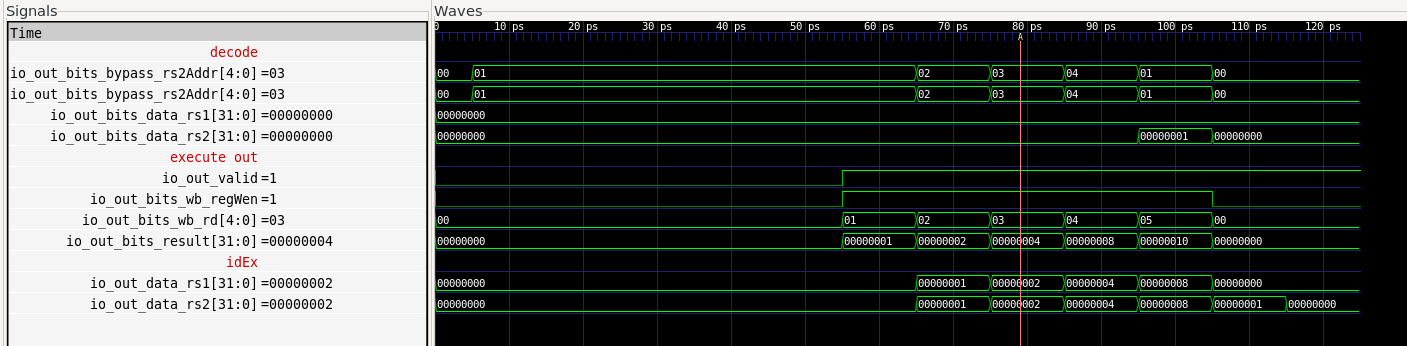
\includegraphics[width=\textwidth]{report_assets/hazard_raw.png}
  \caption{RAW early forwarding 波形：Decode 原始寄存器读值滞后，ID/EX 入队操作数由 EX 组合结果旁路修正}
  \label{fig:hazard-raw}
\end{figure}

图 \ref{fig:hazard-raw} 对应 \texttt{hazard\_raw} 程序。连续 ALU RAW 链中，Decode 阶段从寄存器堆读出的 \texttt{rs1/rs2} 仍可能是旧值或 0，这是因为前序 ALU 指令尚未写回寄存器堆。CourseCPU 在 Decode 到 ID/EX 入队之间加入 early forwarding mux，当 Execute 当前结果的 \texttt{rd} 命中 Decode 指令的 \texttt{rs1Addr/rs2Addr} 时，直接用 \texttt{execute.result} 覆盖 \texttt{idEx.enq.rs1/rs2}。因此波形中可见 ID/EX 入队操作数随 EX 组合输出后一拍更新，证明 ALU-to-ALU RAW 未通过停顿解决，而是通过旁路解决。

\begin{figure}[H]
  \centering
  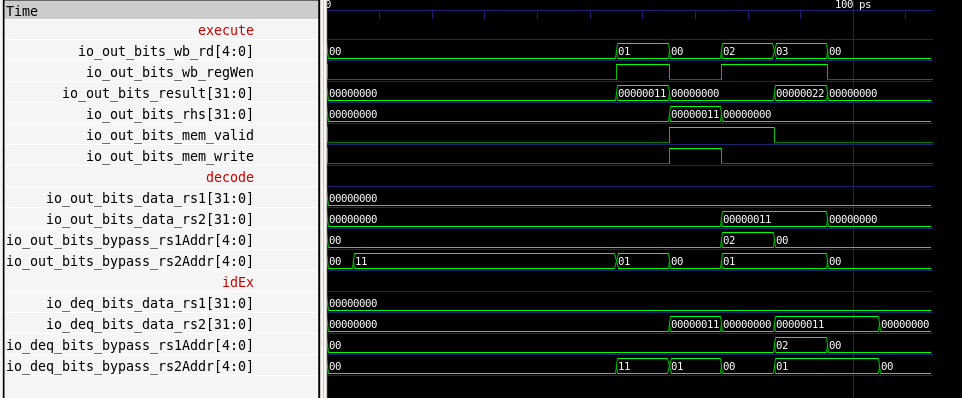
\includegraphics[width=\textwidth]{report_assets/hazard_load_use.png}
  \caption{Load-use 冒险波形：load 指令后继使用者经停顿与 forwarding 获得正确数据}
  \label{fig:hazard-load-use}
\end{figure}

图 \ref{fig:hazard-load-use} 对应 \texttt{hazard\_load\_use} 程序。load 指令进入后端时，\texttt{mem.valid} 有效且 \texttt{mem.write} 为低，说明当前指令为 load。紧随其后的 dependent instruction 在数据尚未写回寄存器堆时需要该值，因此 HazardUnit 触发 load-use stall，随后 load result 通过 \texttt{CourseOperandForward} 在进入 Execute 前转发到操作数路径。波形中 Decode 原始读值尚未更新，但 ID/EX/Execute 侧使用到的 operand 已被转发值修正。

\begin{figure}[H]
  \centering
  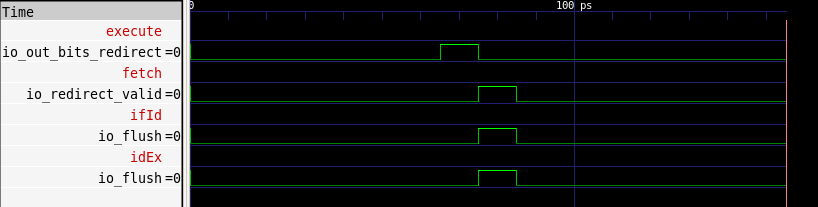
\includegraphics[width=\textwidth]{report_assets/hazard_flush.png}
  \caption{控制冒险 flush 波形：EX 解析 redirect 后前端 PC 修正并清空错误路径流水级}
  \label{fig:hazard-flush}
\end{figure}

图 \ref{fig:hazard-flush} 对应 \texttt{hazard\_flush} 程序。Execute 阶段计算出 redirect 后，Fetch 级 redirect valid 被拉高，IF/ID 与 ID/EX 级的 flush 信号同步清空错误路径指令。该波形展示了控制冒险恢复流程：后端给出正确目标地址，前端 PC 更新，错误路径 valid 被清除，最终错误路径指令不会进入提交点。

\chapter{验证结果}

\section{指令级回归测试}

CourseCPU 通过 directed instruction regression 覆盖 RV32I 基础指令行为，包括算术逻辑、移位、比较、分支、跳转、load/store 和地址生成。Decode、Execute、WriteBack、Fetch 等模块也有独立单元测试，用于在模块粒度定位问题。

\begin{table}[htbp]
  \centering
  \caption{指令级与模块级测试概览}
  \begin{tabularx}{\textwidth}{lXX}
    \toprule
    测试类别 & 覆盖内容 & 状态 \\
    \midrule
    DecodeSpec & 指令译码、控制信号、CSR/SYS 裁剪 & 通过 \\
    CourseCoreRv32iSpec & RV32I 基础程序与组合指令行为 & 通过 \\
    CourseCoreHazardStressSpec & RAW、load-use、flush & 通过 \\
    CourseCoreTraceConfigSpec & trace 配置兼容性 & 通过 \\
    \bottomrule
  \end{tabularx}
\end{table}

\section{Hazard Stress Tests}

Hazard stress tests 重点验证流水线冒险机制。测试包含密集 RAW forwarding chain、load-use stall 以及 branch/JAL flush。通过这些测试可以证明 CourseCPU 不依赖插入大量保守 stall 来保证正确性，而是使用 forwarding 和精确 flush 提升流水线效率。

RTL 兼容 testbench 中将 Scala 侧 \texttt{CourseCoreSmokeSpec}、\texttt{CourseCoreHazardStressSpec}、\texttt{CourseCoreProgramSpec} 和 \texttt{CourseCoreRv32iSpec} 翻译为 9 个 \texttt{.mem} 程序，并为每个程序提供同名 \texttt{.S} 汇编源文件。所有程序均通过同一个 \texttt{tb\_CourseCompatibleTop.sv} 运行并检查寄存器或内存结果。测试集合包括：

\begin{itemize}
  \item \texttt{smoke}：综合算术、访存、分支和跳转。
  \item \texttt{hazard\_raw}：连续 ALU RAW forwarding。
  \item \texttt{hazard\_load\_use}：load-use stall 与 load forwarding。
  \item \texttt{hazard\_flush}：branch/JAL redirect 与错误路径 flush。
  \item \texttt{program\_arith\_upper} 与 \texttt{program\_mem\_byte\_half}：程序级算术与访存 directed case。
  \item \texttt{rv32i\_upper\_jump}、\texttt{rv32i\_alu\_branch}、\texttt{rv32i\_load\_store}：RV32I 指令组合覆盖。
\end{itemize}

\section{真实程序验证}

CourseCPU 能够运行由 RISC-V GCC 编译得到的真实 ELF 程序。报告中重点列出：

\begin{itemize}
  \item \texttt{add-longlong}：覆盖 64-bit 软件整数运算、进位传播和基础函数调用路径。
  \item \texttt{bubble-sort}：覆盖双重循环、数组 load/store、数据相关分支和重复写回。
  \item \texttt{quick-sort}：覆盖递归划分、不规则分支、数组访问、函数调用和栈操作。
  \item \texttt{recursion}：覆盖间接函数调用、递归返回、栈压力和运行时 helper 例程。
  \item \texttt{select-sort}：覆盖选择排序中的嵌套循环、比较分支和数组交换访存。
\end{itemize}

这些程序比单条指令 directed test 更能暴露真实处理器问题。例如排序程序中大量比较和分支会放大控制冒险开销，数组 load/store 会覆盖访存路径，递归和间接调用会覆盖 JAL/JALR、栈访问和返回路径。它们共同构成当前 performance 测试集，也是本报告 IPC、flush probability 和 PPA 摘要的主要性能数据来源。

\section{Difftest 结果}

在真实程序运行过程中，CourseCPU 每条提交指令均与 NEMU reference model 对拍。若出现 PC、寄存器或访存副作用不一致，仿真框架会在错误首次出现处停止并输出相关 trace。当前验证流程中，核心 directed tests 和真实程序均通过 difftest。

\section{覆盖率总结}

覆盖率从三个层面给出：

\begin{itemize}
  \item 指令覆盖：通过 RV32I directed regression 覆盖基础指令类型。
  \item 冒险覆盖：通过 hazard stress tests 覆盖 RAW forwarding、load-use stall 和 branch flush。
  \item 真实程序覆盖：通过 add-longlong、bubble-sort、quick-sort、recursion 和 select-sort 等真实 ELF 程序覆盖复杂控制流、函数调用、递归、栈和数据访存。
\end{itemize}

\begin{table}[htbp]
  \centering
  \caption{覆盖率证据汇总}
  \begin{tabularx}{\textwidth}{lXX}
    \toprule
    覆盖项目 & 证据来源 & 结果 \\
    \midrule
    RV32I 指令覆盖 & Directed regression / difftest / RTL readmem & 通过 \\
    RAW forwarding & Hazard stress test / Vivado waveform & 覆盖 \\
    Load-use stall & Hazard stress test / Vivado waveform & 覆盖 \\
    Branch flush & Hazard stress test / Vivado waveform & 覆盖 \\
    真实程序 & add-longlong, bubble-sort, quick-sort, recursion, select-sort & 通过 \\
    \bottomrule
  \end{tabularx}
\end{table}

\chapter{FPGA 实现与 PPA}

\section{实现环境}

CourseCPU 使用 Vivado 进行综合与实现。RTL 由 Chisel/CIRCT 生成 SystemVerilog，再导入 Vivado 工程。时钟约束设置为 10 ns，对应目标频率 100 MHz。本报告重点记录实现后的 timing、utilization 和 power 结果，并围绕最终关键路径分析 RTL 结构与 FPGA routing 行为。

\section{Timing Summary}

当前最终版本的 timing report 显示 WNS 为 1.255 ns，TNS 为 0，所有用户指定时序约束均满足。在 10 ns 时钟约束下，这表示设计满足 100 MHz 目标，并具有 1.255 ns 正 slack。若按 setup slack 做一阶估算，关键路径等效周期约为 $10 - 1.255 = 8.745$ ns，因此估算 Fmax 为：

\[
  F_{\max} \approx \frac{1000}{10 - 1.255} = 114.35\ \text{MHz}
\]

需要注意的是，该 Fmax 是基于当前 100 MHz 约束和 WNS 的估算值，用于报告中给出直观性能余量；若要得到严格的最高工作频率，仍需要在 Vivado 中逐步收紧时钟约束并重新综合/实现。

\begin{table}[htbp]
  \centering
  \caption{Timing 结果记录}
  \begin{tabularx}{\textwidth}{lXX}
    \toprule
    项目 & 数值 & 说明 \\
    \midrule
    Clock Constraint & 10 ns & 100 MHz 目标约束 \\
    Final WNS & 1.255 ns & TNS = 0，满足所有 setup 约束 \\
    Estimated Fmax & 114.35 MHz & $1000/(10-1.255)$，基于 WNS 的一阶估算 \\
    Final WHS & 0.140 ns & THS = 0，满足 hold 约束 \\
    Total Endpoints & 2961 & sys\_clk 单时钟域 \\
    Critical Path Source & \texttt{exWb} replicated register & \texttt{\_rep\_\_6}/\texttt{\_rep\_\_7} \\
    Critical Path Sink & \texttt{idEx} operand register & data rs1/rs2 写入路径 \\
    \bottomrule
  \end{tabularx}
\end{table}

\section{资源利用率}

最终 Vivado utilization report 显示，CourseCPU 使用 1796 个 Slice LUT 和 1521 个 Slice Register。在目标 FPGA 上 LUT 利用率为 22.45\%，寄存器利用率为 9.51\%。设计未使用 BRAM 和 DSP，说明当前综合配置中的 core 逻辑主要由 LUT、寄存器、MUXF 和 CARRY4 组成。

CourseCPU 在优化过程中显著降低了资源使用。裁剪 CSR/SYS 逻辑后，LUT 曾从约 1999 降至约 1708，FF 从约 1510 降至约 1455。最终版本重新加入 Fetch 级分支预测、trace sideband 和 \texttt{max\_fanout} 复制后，资源回升到 1796 LUT / 1521 FF，但仍保持在较小规模。

\begin{table}[htbp]
  \centering
  \caption{资源利用率对比记录}
  \begin{tabularx}{\textwidth}{lXXXX}
    \toprule
    配置 & LUT & FF & BRAM & 说明 \\
    \midrule
    早期版本 & 约 1999 & 约 1510 & 0 & 未裁剪 CSR/SYS \\
    CSR/SYS 裁剪后 & 约 1708 & 约 1455 & 0 & 面积显著下降 \\
    Final & 1796 & 1521 & 0 & Fetch predictor + max\_fanout 最终配置 \\
    \bottomrule
  \end{tabularx}
\end{table}

\section{功耗估计}

Vivado Power Analysis 估计总片上功耗为 0.113 W，其中动态功耗为 0.054 W，器件静态功耗为 0.059 W。功耗报告 confidence level 为 Low，原因是未提供完整 simulation activity file，I/O 和内部节点翻转率主要来自工具估计。因此该数据适合作为课程报告中的量级参考，而不应视为精确板级功耗。

\begin{table}[htbp]
  \centering
  \caption{Vivado 功耗估计}
  \begin{tabularx}{\textwidth}{lXX}
    \toprule
    项目 & 数值 & 说明 \\
    \midrule
    Total On-Chip Power & 0.113 W & Vivado power report \\
    Dynamic Power & 0.054 W & clocks、logic、signals、I/O 动态功耗 \\
    Device Static Power & 0.059 W & 器件静态功耗 \\
    Junction Temperature & 25.6 $^\circ$C & 默认环境与活动率估计 \\
    Confidence Level & Low & 未提供完整 SAIF/VCD 活动文件 \\
    \bottomrule
  \end{tabularx}
\end{table}

\section{关键路径分析}

最终关键路径显示路径源为 EX/WB stage 中被复制的 \texttt{wb\_rd} 寄存器，例如 \texttt{bitsReg\_wb\_rd\_reg[0]\_rep\_\_6}，终点为 ID/EX stage 中的 operand payload register，例如 \texttt{bitsReg\_data\_rs1\_reg[29]} 或 \texttt{bitsReg\_data\_rs2\_reg[29]}。

该路径逻辑级数约 16 级，其中 routing delay 占比约 60\%。这说明瓶颈并非单纯由某个复杂组合逻辑造成，而是由 forwarding/writeback 相关控制信号在多个区域之间传播导致的 routing-dominated timing。针对这一特点，CourseCPU 使用 \texttt{max\_fanout} 属性引导 Vivado 复制高扇出寄存器，从而改善布线延迟。

\chapter{优化过程}

\section{CSR/SYS 裁剪}

Course 配置不要求完整 CSR 指令、ECALL、EBREAK 等系统指令支持。早期设计中保留这些逻辑会引入额外控制路径、CSR 状态和异常处理 mux，增加 LUT/FF 并影响关键路径。

优化后，CourseCPU 在 DecodePacket 和 Decode 逻辑中加入 \texttt{enableSys} 与 \texttt{enableSimEbreak} 配置。Course 配置下关闭 CSR/SYS 逻辑，同时保留仿真所需的 sim ebreak。该优化使 LUT 和 FF 都明显下降，并改善了 WNS。

\section{Forwarding 策略优化}

CourseCPU 曾尝试多种 forwarding 位置。若将过多写回路径直接拉回 Decode，会增加从 EX/WB 到 ID/EX payload register 的组合路径长度，并造成严重 routing 压力。最终设计将 forwarding 分为两部分：非 load 的 execute result 采用 early forwarding，load result 则通过进入 Execute 前的 CourseOperandForward 处理。

这种划分避免了对所有写回值都建立过宽的回传路径，同时仍然覆盖常见 RAW 数据相关。

\section{Fetch 级分支预测优化}

早期设计中，控制流主要依赖后端 EX 阶段解析，预测收益有限。优化后，GShare predictor 被放入 Fetch 阶段，Fetch 根据当前 instruction 对 branch/JAL 进行预测和目标计算，使前端可以在预测 taken 时直接跳转。

这一优化将 IPC 从约 0.75 提升到约 0.84。相比 BTB 方案，Fetch 级轻量预测面积更小，结构更清晰，也更适合当前 CourseCPU 的规模。

\section{BTB 尝试与回退}

实验过程中曾尝试加入 BTB 缓存分支目标。BTB 能够避免每次都重新计算部分目标，但会增加表项存储、tag/valid 判断和前端控制逻辑。对于当前 CourseCPU 的 benchmark 和 FPGA 资源约束，BTB 带来的 IPC 收益与面积代价不成比例。

因此最终版本移除了较重的 BTB 方案，保留 Fetch 级 GShare predictor 和直接目标计算。这一选择体现了面积、时序和性能之间的工程权衡。

\section{\texttt{max\_fanout} Routing 优化}

Timing report 显示关键路径长期受 routing delay 主导，且源头集中在 EX/WB payload register 的 \texttt{wb\_rd} 等高扇出信号。简单调整 RTL 表达式并不能稳定改变 Vivado 的物理布局，因此 CourseCPU 在 \texttt{FlushableStage} 中加入可选 \texttt{maxFanout} 参数，并仅对 EX/WB stage 启用。

最终配置为：

\begin{lstlisting}[language={}]
val exWb = Module(
  new FlushableStage(
    new ExecutePacket(enableTraceFields),
    maxFanout = Some(4)
  )
)
\end{lstlisting}

生成的 SystemVerilog 中出现 \texttt{(* max\_fanout = 4 *)} 属性，Vivado 实现后 timing report 中出现 \texttt{\_rep\_\_6}、\texttt{\_rep\_\_7} 等复制寄存器，说明优化被综合和布局布线工具实际采用。该优化将 WNS 提升到约 1.255 ns。

\section{优化对比}

\begin{table}[htbp]
  \centering
  \caption{CourseCPU 优化过程摘要}
  \begin{tabularx}{\textwidth}{lXXXX}
    \toprule
    阶段 & IPC & LUT & FF & WNS \\
    \midrule
    Baseline & 约 0.69--0.75 & 约 1999 & 约 1510 & 约 0.7--1.1 ns \\
    CSR/SYS 裁剪 & 约 0.75 & 约 1708 & 约 1455 & 约 1.349 ns \\
    Fetch Predictor & 约 0.84 & 约 1800 & 约 1500 & 约 1.0 ns 级 \\
    \texttt{max\_fanout=8} & 约 0.84 & 约 1800 & 约 1500 & 约 1.247 ns \\
    \texttt{max\_fanout=4} & 约 0.84 & 1796 & 1521 & 1.255 ns \\
    \bottomrule
  \end{tabularx}
\end{table}

\chapter{设计分析与讨论}

\section{真实 ELF + Difftest 的价值}

传统课程实验常使用手写 \texttt{.mem} 程序和简单 testbench 检查最终结果。这种方式可以证明某些 directed case 通过，但难以覆盖真实程序中的复杂交互。CourseCPU 的验证环境使用 RISC-V GCC、ELF loader、abstract-machine SDK、Verilator 和 NEMU difftest，使测试对象从“几条指令”提升到“真实软件栈”。

这种验证方式能够覆盖函数调用、栈、全局数据、循环、递归、访存模式和复杂控制流，也能够在每条 commit 指令处检查架构状态。因此，CourseCPU 的验证可信度显著高于只看最终内存结果的方式。

\section{分支预测的收益与代价}

CourseCPU 的分支预测优化说明，真实程序性能不仅取决于 ALU 或访存是否正确，还取决于控制流处理效率。Fetch 级 GShare predictor 在较小面积下提升 IPC，而 BTB 虽然理论上能进一步降低目标计算开销，但对当前规模的 core 而言面积和 routing 代价较高。

因此最终设计选择较轻量的 predictor。这种选择不是功能不足，而是基于 workload、面积和时序的工程权衡。

\section{FPGA Timing 的经验}

CourseCPU 的 timing 优化过程表明，FPGA 上的关键路径不总是由 RTL 中看起来最复杂的逻辑决定。即使逻辑级数没有明显增加，routing delay 也可能由于 fanout、布局距离和信号复制策略而成为主导。

对于 routing-dominated path，简单重写 \texttt{Mux} 或拆分 \texttt{when} 语句往往收益有限。更有效的方法是向综合/实现工具提供物理实现相关信息，例如 \texttt{max\_fanout}，使工具进行寄存器复制或局部优化。

\section{当前限制与后续方向}

CourseCPU 当前仍是单发射顺序 core，没有 cache，也没有完整异常/中断/CSR 系统。Fetch predictor 采用轻量设计，未保留最终 BTB。后续可以考虑：

\begin{itemize}
  \item 加入 I-cache/D-cache，提升真实程序访存性能。
  \item 引入更系统的 branch predictor 和 BTB，并重新评估面积收益比。
  \item 增强性能计数器，统计 branch hit rate、load-use stall count 等。
  \item 在 Vivado 中加入更完整的 XDC 约束、物理优化策略和 floorplan 实验。
  \item 支持完整 CSR、异常和中断，向更完整的系统级 CPU 演进。
\end{itemize}

\chapter{总结}

CourseCPU 实现了一个完整的 RV32I 四级流水线处理器系统。它不仅完成了基础指令执行、流水线冒险处理和 FPGA 综合实现，还建立了基于真实 RISC-V GCC ELF 程序、Verilator 周期级仿真和 NEMU difftest 的验证平台。

在功能方面，CourseCPU 支持 RV32I 整数指令级功能，并能够运行 \texttt{add-longlong}、\texttt{bubble-sort}、\texttt{quick-sort}、\texttt{recursion}、\texttt{select-sort} 等真实 C 程序。在微架构方面，它采用单发射顺序四级流水线，包含 forwarding、load-use stall、flush recovery 和 Fetch 级 GShare branch predictor。在验证方面，它使用 commit trace 与 reference model 对拍，提供比传统 directed test 更高的可信度。

在 FPGA 实现方面，CourseCPU 通过 CSR/SYS 裁剪、branch predictor 精简和 \texttt{max\_fanout} register replication 优化面积与时序。最终 timing report 显示设计满足 10 ns 时钟约束，并获得约 1.255 ns 的正 slack。

总体而言，CourseCPU 是一个面向真实软硬件协同环境的教学型 CPU 产品原型。它的价值不仅在于完成 RV32I core 本身，更在于构建了一套接近工业 CPU 开发流程的设计、验证和优化闭环。

\appendix

\chapter{RV32I 指令支持表}

\begin{longtable}{>{\bfseries}l p{0.7\textwidth}}
  \caption{CourseCPU RV32I 指令支持表}\\
  \toprule
  类型 & 指令 \\
  \midrule
  算术逻辑 & ADD, SUB, AND, OR, XOR, ADDI, ANDI, ORI, XORI \\
  移位 & SLL, SRL, SRA, SLLI, SRLI, SRAI \\
  比较 & SLT, SLTU, SLTI, SLTIU \\
  分支 & BEQ, BNE, BLT, BGE, BLTU, BGEU \\
  跳转 & JAL, JALR \\
  访存 & LB, LH, LW, LBU, LHU, SB, SH, SW，以及 byte-addressed memory 相关路径 \\
  地址生成 & LUI, AUIPC \\
  \bottomrule
\end{longtable}

\chapter{关键模块接口说明}

\begin{itemize}
  \item \texttt{CourseCore}：CPU 顶层，连接 IMEM、DMEM、debug、trace 和各流水级模块。
  \item \texttt{Fetch}：维护 PC，访问 IMEM，执行 Fetch 级分支预测。
  \item \texttt{Decode}：完成译码、寄存器读取、立即数生成和控制信号生成。
  \item \texttt{Execute}：完成 ALU、分支解析、访存地址生成和 redirect 生成。
  \item \texttt{WriteBack}：完成 load 数据处理、寄存器写回和 commit trace。
  \item \texttt{FlushableStage}：通用流水线寄存器，支持 valid/ready 和 flush。
  \item \texttt{Tracer}：输出 commit trace、统计 IPC 和 flush count，并可接入 DPI。
\end{itemize}

\chapter{仿真运行命令示例}

\begin{lstlisting}[language={}]
# 生成 Course 仿真 RTL 并构建 Verilator 仿真器
make -C course-sim

# 运行真实 benchmark 程序，不开启 difftest
make -C course-sim run IMG=../reports/performance/quick-sort/quick-sort-riscv32e-npc.bin

# 运行真实 benchmark 程序，并接入 NEMU reference model 进行 difftest
make -C course-sim rundiff IMG=../reports/performance/quick-sort/quick-sort-riscv32e-npc.bin
\end{lstlisting}

\begin{lstlisting}[language={}]
# 运行 CourseCore 相关 Scala/Chisel 测试
sbt -Dsbt.server=false --batch \
  "testOnly labcpu.core.CourseCoreRv32iSpec \
            labcpu.core.CourseCoreHazardStressSpec \
            labcpu.core.CourseCoreTraceConfigSpec \
            mycpu.core.backend.DecodeSpec"
\end{lstlisting}

\begin{lstlisting}[language={}]
# 生成 CourseCompatibleTop，并运行 readmemh RTL 兼容测试
bash src/test/verilog/course_compat/run_course_compat_tests.sh

# 为单个程序导出局部 VCD 波形，用 GTKWave 或 Vivado 打开
bash src/test/verilog/course_compat/dump_course_compat_wave.sh \
  hazard_load_use 0 20
\end{lstlisting}

\chapter{RTL 兼容测试程序清单}

\begin{table}[htbp]
  \centering
  \caption{readmemh RTL 兼容测试程序}
  \begin{tabularx}{\textwidth}{lXX}
    \toprule
    程序 & 源文件 & 覆盖目标 \\
    \midrule
    smoke & \texttt{smoke.S}/\texttt{smoke.mem} & 算术、访存、分支、跳转综合 smoke test \\
    hazard\_raw & \texttt{hazard\_raw.S}/\texttt{hazard\_raw.mem} & 连续 ALU RAW early forwarding \\
    hazard\_load\_use & \texttt{hazard\_load\_use.S}/\texttt{hazard\_load\_use.mem} & load-use stall 与 load forwarding \\
    hazard\_flush & \texttt{hazard\_flush.S}/\texttt{hazard\_flush.mem} & branch/JAL redirect 与错误路径 flush \\
    program\_arith\_upper & \texttt{program\_arith\_upper.S}/\texttt{program\_arith\_upper.mem} & LUI、移位、ALU、LW/SW 组合程序 \\
    program\_mem\_byte\_half & \texttt{program\_mem\_byte\_half.S}/\texttt{program\_mem\_byte\_half.mem} & SB/LBU/SH/LHU 字节和半字访存 \\
    rv32i\_upper\_jump & \texttt{rv32i\_upper\_jump.S}/\texttt{rv32i\_upper\_jump.mem} & U/J/I-type 指令与 JAL/JALR \\
    rv32i\_alu\_branch & \texttt{rv32i\_alu\_branch.S}/\texttt{rv32i\_alu\_branch.mem} & R-type ALU 与六类 branch \\
    rv32i\_load\_store & \texttt{rv32i\_load\_store.S}/\texttt{rv32i\_load\_store.mem} & LB/LH/LW/LBU/LHU/SB/SH/SW \\
    \bottomrule
  \end{tabularx}
\end{table}

这些程序均由同一个 \texttt{tb\_CourseCompatibleTop.sv} 驱动。测试通过 \texttt{+IMEM=<path>} 装载 \texttt{.mem}，通过 \texttt{+TEST=<name>} 选择期望检查，不需要为每个程序编写独立 testbench。

\chapter{代表性程序运行统计}

\begin{table}[htbp]
  \centering
  \caption{代表性程序运行统计}
  \begin{tabular}{lrrrr}
    \toprule
    程序 & Cycles & Instructions & IPC & Flush Probability \\
    \midrule
    add-longlong & 1889 & 1640 & 0.868184 & 0.050000 \\
    bubble-sort & 3792 & 3156 & 0.832278 & 0.066857 \\
    quick-sort & 3904 & 3304 & 0.846311 & 0.060230 \\
    recursion & 9172 & 6550 & 0.714130 & 0.133282 \\
    select-sort & 4126 & 3655 & 0.885846 & 0.042681 \\
    \midrule
    加权汇总 & 22883 & 18305 & 0.799939 & 0.083092 \\
    \bottomrule
  \end{tabular}
\end{table}

\chapter{Performance Benchmark C 源码}

本附录列出 performance 测试集中用于生成 ELF benchmark 的 C 源码。这些程序经 RISC-V GCC 与 Abstract-Machine 运行时编译链接后，由 Verilator 仿真平台装载执行，并参与正文中的 IPC 与 flush probability 统计。

\begin{table}[htbp]
  \centering
  \caption{Performance benchmark 源码清单}
  \begin{tabularx}{\textwidth}{lX}
    \toprule
    程序 & Workload 特征 \\
    \midrule
    add-longlong & 64-bit 软件整数加法与进位传播 \\
    bubble-sort & 双重循环、数组 load/store 与数据相关分支 \\
    quick-sort & 递归快速排序、不规则分支与栈访问 \\
    recursion & 间接递归调用链、返回路径与运行时 helper 压力 \\
    select-sort & 选择排序循环、比较分支与数组交换访存 \\
    \bottomrule
  \end{tabularx}
\end{table}

\section{\texttt{add-longlong.c}}

\lstinputlisting[language=C,caption={add-longlong benchmark 源码}]{report_assets/add-longlong.c}

\section{\texttt{bubble-sort.c}}

\lstinputlisting[language=C,caption={bubble-sort benchmark 源码}]{report_assets/bubble-sort.c}

\section{\texttt{quick-sort.c}}

\lstinputlisting[language=C,caption={quick-sort benchmark 源码}]{report_assets/quick-sort.c}

\section{\texttt{recursion.c}}

\lstinputlisting[language=C,caption={recursion benchmark 源码}]{report_assets/recursion.c}

\section{\texttt{select-sort.c}}

\lstinputlisting[language=C,caption={select-sort benchmark 源码}]{report_assets/select-sort.c}

\chapter{Vivado 报告摘录}

\section{Timing Report 摘录}

最终关键路径示例：

\begin{lstlisting}[language={}]
Slack (MET) : 1.255ns
Source:      core/exWb/payload/bitsReg_wb_rd_reg[0]_rep__6/C
Destination: core/idEx/payload/bitsReg_data_rs1_reg[29]/D
Data Path Delay: 8.609ns
Logic Levels: 16
\end{lstlisting}

\section{Utilization Report 摘录}

\begin{lstlisting}[language={}]
Slice LUTs:       1796 / 8000   (22.45%)
Slice Registers:  1521 / 16000  (9.51%)
Block RAM Tile:      0 / 20     (0.00%)
DSPs:                0 / 40     (0.00%)
BUFGCTRL:            1 / 32     (3.13%)
\end{lstlisting}

\section{Power Report 摘录}

\begin{lstlisting}[language={}]
Total On-Chip Power: 0.113 W
Dynamic Power:       0.054 W
Device Static Power: 0.059 W
Confidence Level:    Low
\end{lstlisting}

\end{document}
